\documentclass[a4paper]{article}
\usepackage[french]{babel}
\usepackage[T1]{fontenc}
\usepackage[utf8]{inputenc}
\usepackage{authblk}
\usepackage{url}
\usepackage{hyperref}
\usepackage{amsmath}
\usepackage{tcolorbox}
\usepackage{tikz} 
\usepackage[nottoc,numbib]{tocbibind}

\title{100-prisonniers}
\date{27/11/2023}

\author{GUETTEVILLE Nathan}
\author{LACENNE Yanis}
\author{SOAN Tony Ly}

\affil{G4S12}

\renewcommand\Authands{ et }
\begin{document}

\maketitle

\pagenumbering{gobble}
\pagenumbering{arabic}

\tableofcontents

\newpage

\section{Introduction}

Le problème des 100 prisonniers \cite{100PrisonersProblem2023} se présente
comme suit:
"le directeur d'une prison décide d'offrir une chance d'être libéré à 100 prisonniers
condamnés à mort sous la forme d'une épreuve.
Chacun d'eux porte un uniforme numéroté de 1 à 100, et dans 100 boîtes distinctes
numérotées de 1 à 100 fermées, chacune contient un papier avec le numéro d'un
prisonnier correspondant écrit dessus.
Les papiers sont répartis aléatoirement dans les boîtes et elles sont placées dans une
salle isolée.

Les prisonniers doivent y entrer tour à tour et seuls.
Après le passage de chaque prisonnier, la salle est remise à l'état initial.

Lors du passage dans cette salle, chacun d'eux à le droit d'ouvrir
et de regarder dans 50 boîtes au plus,

\begin{itemize}
	\item
	      si durant son tour un prisonnier parvient à trouver son propre numéro
	      dans une boite, il peut alors quitter la salle.
	\item
	      s'il ne parvient pas à trouver son propre numéro, alors tous les
	      prisonniers sont exécutés.
\end{itemize}

Les prisonniers ne peuvent pas communiquer entre eux durant l'épreuve,
mais il peuvent établir une stratégie avant qu'elle ne commence."\\\\
Ce problème présenté \cite{veritasiumRiddleThatSeems2022} par
\href{https://www.veritasium.com/about}{Derek Muller}
(alias \href{https://www.youtube.com/@veritasium}{Veritasium})
est une version modifiée du problème
initial \cite{miltersenCellProbeComplexity2007} formulé par
\href{https://pure.au.dk/portal/en/persons/bromille%40cs.au.dk}{Peter Bro Miltersen}
, et de la version \cite{flajoletAnalyticCombinatorics2009} de
\href{https://fr.wikipedia.org/wiki/Philippe_Flajolet}{Philippe Flajolet}
et \href{https://sedgewick.io/}{Robert Sedgewick}.


\section{Lien avec les mathématiques discrètes}

\subsection{Permutations}

	\begin{tcolorbox}
		En mathématiques, la notion de \href{https://fr.wikipedia.org/wiki/Permutation}{permutation} exprime l'idée de réarrangement d'objets discernables. Une permutation d'objets distincts rangés dans un certain ordre correspond à un changement de l'ordre de succession de ces objets.
		\par
	\end{tcolorbox}

	On rappelle de fait qu'il existe $n!$ moyens d'ordonner $n$ éléments distincts.
	Considérons la permutation suivante qui envoie $1$ vers $4$, $2$ vers $1$, $3$ vers lui-même et $4$ vers $2$.

	\begin{center}
		\label{example1}
		$1 \longrightarrow 4$ \\
		$2 \longrightarrow 1$ \\
		$3 \longrightarrow 3$ \\
		$4 \longrightarrow 2$ \\
	\end{center}

	Il est tout à fait possible de représenter une permutation sous forme de graphe.

	\begin{center}
		\begin{tikzpicture}[main/.style = {draw, circle}]
			\node[main] (1) {$1$};
			\node[main] (2) [right of=1] {$2$};
			\node[main] (4) [below of=1] {$4$};
			\node[main] (3) [below of=2] {$3$};

			\draw [arrows=->] (1) to (4);
			\draw[arrows=->] (4) .. controls +(up:3mm) and +(down:7mm) .. (2);
			\draw[->] (2) -- (1);
			\draw[->] (3) .. controls +(up:7mm) and +(right:7mm) .. (3);
			(3);
		\end{tikzpicture}
	\end{center}

	En voici un exemple plus poussé contenant 100 noeuds.

	\begin{center}
		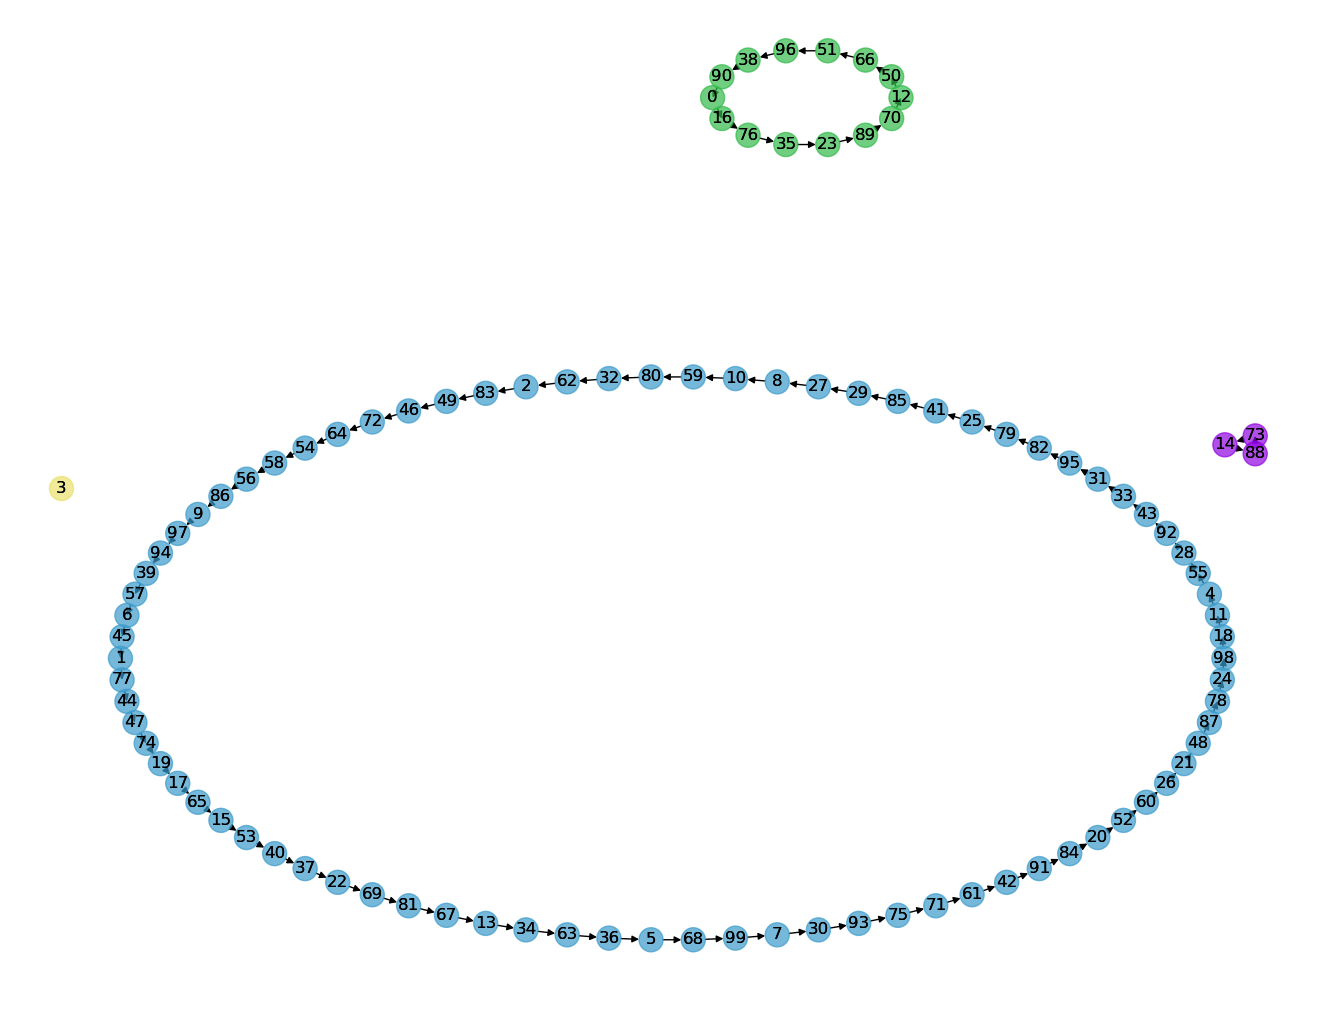
\includegraphics[scale=0.4]{Figure_1}
	\end{center}

\subsection{Cycles d'une permutation}

	On souhaite maintenant considérer les cycles contenus dans les permutations.
	En continuant avec notre exemple, on remarque que notre permutation contient 2 cycles.
	Un cycle de longueur 3 $(1 \rightarrow 4 \rightarrow 2 \rightarrow 1)$ et un de longueur 1 $(3 \rightarrow 3)$.
	Sauf que, nous pouvons également remarquer que le cycle $(1 \rightarrow 4 \rightarrow 2 \rightarrow 1)$ est le même que $(4 \rightarrow 2 \rightarrow 1 \rightarrow 4)$ et $(2 \rightarrow 1 \rightarrow 4 \rightarrow 2)$. \\
	Il y a $3! = 6$ manières d'écrire une permutation de 3 éléments.
	Toutefois, on vient de dire qu'un cycle de 3 éléments pouvait s'écrire de 3 façons différentes; alors parmi ces $6$ permutations, il n'existe que $\frac{6}{3} = 2$ cycles distincts.
	\begin{align*}
		 & A \rightarrow B \rightarrow C \rightarrow A \qquad & A \rightarrow C  \rightarrow B \rightarrow A \\
		 & B \rightarrow C \rightarrow A \rightarrow B \qquad & C \rightarrow B  \rightarrow A \rightarrow C \\
		 & C \rightarrow A \rightarrow B \rightarrow C \qquad & B \rightarrow A  \rightarrow C \rightarrow B
	\end{align*}

	On peut le généraliser pour $n$ en disant qu'il y a $\frac{n!}{n} = (n-1)!$ façons d'écrire un cycle de $n$ éléments. \\

	On cherche maintenant à obtenir la quantité de permutations de $n$ contenant un cycle de longueur $ 0 < k \leq n$.
	Il y en a $\frac{n!}{k}$.

	\begin{align*}
		\binom{n}{k} * (k - 1)! * (n - k)! & = \frac{n!}{k! * (n - k)!} * (k - 1)! * (n - k)!           \\
		                                   & = \frac{n! * (k - 1)! * (n - k)!}{k * (k - 1)! * (n - k)!} \\
		                                   & = \frac{n!}{k}
	\end{align*}

	Avec
	\begin{itemize}
		\item $\binom{n}{k}$ : les éléments formant le cycle
		\item $(k - 1)!$ : le nombre de permutations des éléments formant le cycle
		\item $(n - k)!$ : le nombre de permutations des éléments restants
	\end{itemize}


\section{Probabilités}
\subsection{Problématique}

	Comment se fait-il que les prisonniers aient un pourcentage de chances de s'en sortir d'environ 30\% ? \\

\subsection{Probabilités de cycles}

	Nous avons vu dans la section précédente que le nombre de permutations de $n$ contenant un cycle de longueur $0 < k \leq n$ est de $\frac{n!}{k}$.
	À partir de cette information, nous sommes maintenant capable de calculer la probabilité d'obtenir un cycle de longueur $\frac{n}{2} < k \leq n$ dans une permutation de longueur $n$.
	Nous ne parlerons pas ici de la probabilité de la lorsque $0 < k \leq \frac{n}{2}$.

	Soit les événements aléatoires
	\begin{center}
		$E_k$ : "Une permutation de n contient un cycle de longueur k." \\
		$E'_k$ : "Une permutation de n contient un cycle de longueur au moins k."
	\end{center}

	Muni de la \href{https://fr.wikipedia.org/wiki/Loi_uniforme_discr%C3%A8te#Calcul_d'une_probabilit%C3%A9}{loi uniforme discrète}, on sait que $P(X \in B) = \frac{\#(A \cap B)}{\#A}$, de fait :

	\begin{equation}
		P(E_k) = \frac{\frac{n!}{k}}{n!} = \frac{1}{k}
	\end{equation}

	À partir de $P(E_k)$, on peut désormais aisément calculer $P(E'_k)$ :

	\begin{equation}
		P(E'_k) = \sum_{i = k}^{n} P(E_i) = \sum_{i = k}^{n} \frac{1}{i}
	\end{equation}

	On reconnaît ici une forme de \href{https://en.wikipedia.org/wiki/Harmonic_series_(mathematics)#}{série harmonique}.
	En prenant $k = \frac{n}{2}$, on obtient

	\begin{equation}
		P(E'_{\frac{n}{2}}) = \frac{1}{\frac{n}{2}} + \hdots + \frac{1}{n - 1} + \frac{1}{n}
	\end{equation}

	Il est possible de développer en utilisant la série Harmonique.

	\begin{align*}
		P(E'_{\frac{n}{2}}) & = H(n) - H(\lfloor \frac{n}{2} \rfloor)     \\
		                    & \approx \ln{n} - \ln{\frac{n}{2}}           \\
		                    & \approx \ln{\frac{n}{\frac{n}{2}}} = \ln{2} \\
		                    & \approx 0.693147181
	\end{align*}

	En conclusion, il y a environ 70\% de chances qu'une permutation de $n$ éléments contiennent un cycle d'au moins $\frac{n}{2}$.

\subsection{Interpretation}

	Nous savons que les prisonniers ne peuvent s'en sortir que si le cycle maximal est de $\frac{n}{2}$.
	Ce qui leur laisse environ 30\% de chance de survie.


\section{Baby-Step Giant-Step}
Qu'est-ce que l'algorithme `Baby-Step Giant-Step` ? À quoi sert-il et quel est le lien avec les prisonniers ?

TODO : Nathan

\section{Conclusion}

\section{Annexe}
\begin{itemize}
	\item Permutation des cycles: \url{https://github.com/YanisLcn/100-prisoners/blob/master/tools/permutation_cycles.py}
	\item Programme : Afficher le graphe d'une permutation
	      (TODO : Yanis)
	\item Programme : Tester la probabilité de survie des prisonniers / Comparaison entre la stratégie aléatoire et la stratégie gagnante.
	      (TODO : Nathan)
\end{itemize}

\bibliographystyle{IEEEtran}
\bibliography{citation}

\end{document}
